\iffalse
This file is protected by Copyright. Please refer to the COPYRIGHT file
distributed with this source distribution.

This file is part of OpenCPI <http://www.opencpi.org>

OpenCPI is free software: you can redistribute it and/or modify it under the
terms of the GNU Lesser General Public License as published by the Free Software
Foundation, either version 3 of the License, or (at your option) any later
version.

OpenCPI is distributed in the hope that it will be useful, but WITHOUT ANY
WARRANTY; without even the implied warranty of MERCHANTABILITY or FITNESS FOR A
PARTICULAR PURPOSE. See the GNU Lesser General Public License for more details.

You should have received a copy of the GNU Lesser General Public License along
with this program. If not, see <http://www.gnu.org/licenses/>.
\fi

%----------------------------------------------------------------------------------------
% Update the docTitle and docVersion per document
%----------------------------------------------------------------------------------------
\def\docTitle{OpenCPI\\ FSK Digital Radio Controller App Guide}
\def\docVersion{\color{red}develop} % MAKE SURE THIS MATCHES WHAT THE APP PRINTS w/ --version
%----------------------------------------------------------------------------------------
\documentclass{article}
\iffalse
This file is protected by Copyright. Please refer to the COPYRIGHT file
distributed with this source distribution.

This file is part of OpenCPI <http://www.opencpi.org>

OpenCPI is free software: you can redistribute it and/or modify it under the
terms of the GNU Lesser General Public License as published by the Free Software
Foundation, either version 3 of the License, or (at your option) any later
version.

OpenCPI is distributed in the hope that it will be useful, but WITHOUT ANY
WARRANTY; without even the implied warranty of MERCHANTABILITY or FITNESS FOR A
PARTICULAR PURPOSE. See the GNU Lesser General Public License for more details.

You should have received a copy of the GNU Lesser General Public License along
with this program. If not, see <http://www.gnu.org/licenses/>.
\fi
\author{} % Force author to be blank
%----------------------------------------------------------------------------------------
% Paper size, orientation and margins
%----------------------------------------------------------------------------------------
\usepackage{geometry}
\geometry{
        letterpaper, % paper type
        portrait,    % text direction
        left=.75in,  % left margin
        top=.75in,   % top margin
        right=.75in, % right margin
        bottom=.75in % bottom margin
 }
%----------------------------------------------------------------------------------------
% Header/Footer
%----------------------------------------------------------------------------------------
\usepackage{fancyhdr} \pagestyle{fancy} % required for fancy headers
\renewcommand{\headrulewidth}{0.5pt}
\renewcommand{\footrulewidth}{0.5pt}
\rhead{\small{ANGRYVIPER Team}}
% \rfoot{\thepage}
%----------------------------------------------------------------------------------------
% Appendix packages
%----------------------------------------------------------------------------------------
\usepackage[toc,page]{appendix}
%----------------------------------------------------------------------------------------
% Defined Commands & Renamed Commands
%----------------------------------------------------------------------------------------
\renewcommand{\contentsname}{Table of Contents}
\renewcommand{\listfigurename}{List of Figures}
\renewcommand{\listtablename}{List of Tables}
%----------------------------------------------------------------------------------------
% Various packages
%----------------------------------------------------------------------------------------
\usepackage[usenames,dvipsnames]{xcolor} % for color names see https://en.wikibooks.org/wiki/LaTeX/Colors
\usepackage{hyperref}  % for linking urls and lists
\usepackage{graphicx}  % for including pictures by file
\usepackage{listings}  % for coding language styles
\usepackage{rotating}  % for sideways table
\usepackage{pifont}    % for sideways table
\usepackage{pdflscape} % for landscape view
\usepackage{subfig}
\usepackage{xstring}
\uchyph=0 % Never hyphenate acronyms like RCC (I think this overrides ANGRYVIPER above)
\renewcommand\_{\textunderscore\allowbreak} % Allow words to break/newline on underscores
%----------------------------------------------------------------------------------------
% Table packages
%----------------------------------------------------------------------------------------
\usepackage{longtable} % for long possibly multi-page tables
\usepackage{tabularx} % c=center,l=left,r=right,X=fill
% These define tabularx columns "C" and "R" to match "X" but center/right aligned
\newcolumntype{C}{>{\centering\arraybackslash}X}
\newcolumntype{R}{>{\raggedleft\arraybackslash}X}
\usepackage{float}
\floatstyle{plaintop}
\usepackage[tableposition=top]{caption}
\newcolumntype{P}[1]{>{\centering\arraybackslash}p{#1}}
\newcolumntype{M}[1]{>{\centering\arraybackslash}m{#1}}
%----------------------------------------------------------------------------------------
% Block Diagram / FSM Drawings
%----------------------------------------------------------------------------------------
\usepackage{tikz}
\usetikzlibrary{shapes,arrows,fit,positioning}
\usetikzlibrary{automata} % used for the fsm
%----------------------------------------------------------------------------------------
% Colors Used
%----------------------------------------------------------------------------------------
\usepackage{colortbl}
\definecolor{blue}{rgb}{.7,.8,.9}
\definecolor{ceruleanblue}{rgb}{0.16, 0.32, 0.75}
\definecolor{drkgreen}{rgb}{0,0.6,0}
\definecolor{deepmagenta}{rgb}{0.8, 0.0, 0.8}
\definecolor{cyan}{rgb}{0.0,0.6,0.6}
\definecolor{maroon}{rgb}{0.5,0,0}
%----------------------------------------------------------------------------------------
% VHDL Coding Language Style
% modified from: http://latex-community.org/forum/viewtopic.php?f=44&t=22076
%----------------------------------------------------------------------------------------
\lstdefinelanguage{VHDL}
{
        basicstyle=\ttfamily\footnotesize,
        columns=fullflexible,keepspaces,      % https://tex.stackexchange.com/a/46695/87531
        keywordstyle=\color{ceruleanblue},
        commentstyle=\color{drkgreen},
        morekeywords={
    library,use,all,entity,is,port,in,out,end,architecture,of,
    begin,and, signal, when, if, else, process, end,
        },
        morecomment=[l]--
}
%----------------------------------------------------------------------------------------
% XML Coding Language Style
% modified from: http://tex.stackexchange.com/questions/10255/xml-syntax-highlighting
%----------------------------------------------------------------------------------------
\lstdefinelanguage{XML}
{
        basicstyle=\ttfamily\footnotesize,
        columns=fullflexible,keepspaces,
        morestring=[s]{"}{"},
        morecomment=[s]{!--}{--},
        commentstyle=\color{drkgreen},
        moredelim=[s][\color{black}]{>}{<},
        moredelim=[s][\color{cyan}]{\ }{=},
        stringstyle=\color{maroon},
        identifierstyle=\color{ceruleanblue}
}
%----------------------------------------------------------------------------------------
% DIFF Coding Language Style
% modified from http://tex.stackexchange.com/questions/50176/highlighting-a-diff-file
%----------------------------------------------------------------------------------------
\lstdefinelanguage{diff}
{
        basicstyle=\ttfamily\footnotesize,
        columns=fullflexible,keepspaces,
        breaklines=true,                                % wrap text
        morecomment=[f][\color{ceruleanblue}]{@@},      % group identifier
        morecomment=[f][\color{red}]-,                  % deleted lines
        morecomment=[f][\color{drkgreen}]+,             % added lines
        morecomment=[f][\color{deepmagenta}]{---},      % Diff header lines (must appear after +,-)
        morecomment=[f][\color{deepmagenta}]{+++},
}
%----------------------------------------------------------------------------------------
% Python Coding Language Style
% modified from
%----------------------------------------------------------------------------------------
\lstdefinelanguage{python}
{
        basicstyle=\ttfamily\footnotesize,
        columns=fullflexible,keepspaces,
        keywordstyle=\color{ceruleanblue},
        commentstyle=\color{drkgreen},
        stringstyle=\color{orange},
        morekeywords={
    print, if, sys, len, from, import, as, open,close, def, main, for, else, write, read, range,
        },
        comment=[l]{\#}
}
%----------------------------------------------------------------------------------------
% Fontsize Notes in order from smallest to largest
%----------------------------------------------------------------------------------------
%    \tiny
%    \scriptsize
%    \footnotesize
%    \small
%    \normalsize
%    \large
%    \Large
%    \LARGE
%    \huge
%    \Huge

\date{Version \docVersion} % Force date to be blank and override date with version
\title{\docTitle}
\lhead{FSK Digital Radio Controller App Guide}
%----------------------------------------------------------------------------------------
%\usepackage[T1]{fontenc} % http://tex.stackexchange.com/a/181119
\usepackage{graphicx}
\graphicspath{ {figures/} }
\usepackage{textcomp}
\usepackage{listings}

\begin{document}
\maketitle
%\thispagestyle{fancy}

\begin{center}
  \textit{\textbf{Revision History}}
  \begin{longtable}{|p{2cm}|p{12cm}|p{2.4cm}|}
    \hline
    \rowcolor{blue}
    \textbf{Revision} & \textbf{Description of Change} & \textbf{Date} \\
    \hline
    \docVersion & Initial Release & \color{red}pre-release \\
    \hline
  \end{longtable}
\end{center}

\tableofcontents

\listoffigures

\begin{landscape}

  \section{Description}

    This application is a 2-level FSK modem that is based on the dig\_radio\_ctrlr
    component spec
    which provides a fully RF transceiver-agnostic command/control mechanism for RF
    transceivers.
    The modulation algorithm reads a JPEG file from disk which has been modified to
    include a bit synchronization pattern that the demodulation algorithm's
    real\_digitizer
    worker is hardcoded to
    recognize.

    \subsection{Application Modes}

      The application may be run in either the \textit{filerw}, \textit{rx},
      \textit{tx}, or \textit{txrx} mode.
      The application XML filename is sent as the last argument to the
      application executable. This filename is in the format
      \texttt{<description>\_<mode>.xml}, e.g. \texttt{foo\_txrx.xml} would force
      the executable to use the
      \textit{txrx} mode.
      The \textit{filerw} mode uses file\_read and file\_write workers to
      process the input using only application workers (platform-agnostic) in a
      purely digital fashion.
      The \textit{rx} mode inputs I/Q data from the ADC and processes the FSK
      signal down to bits that are written to file.
      The \textit{tx} mode modulates the input file as a FSK signal, and
      transmits the input via the DAC.
      The \textit{txrx} mode is the full transceiver mode of the application
      which combines the functionality of the \textit{rx} and \textit{tx} modes
      into a single application. This mode transmits input file data as the
      radio RF TX output and inputs RF RX radio input that is written to file.

      {\centering

      \begin{figure}[htpb]
        \centering
        \captionsetup{type=figure}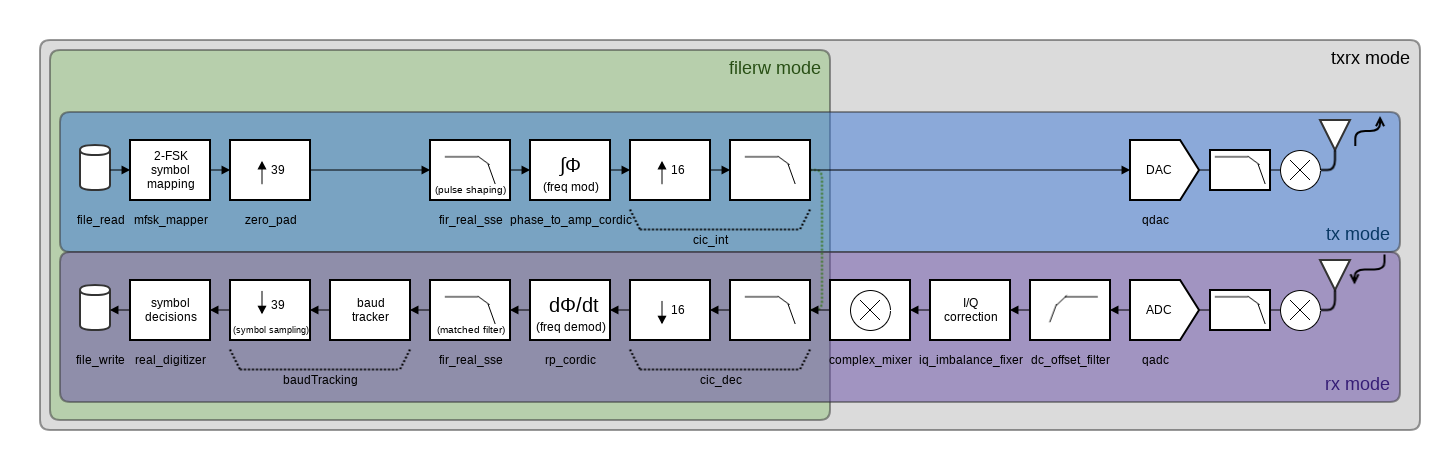
\includegraphics[scale=0.47]{fsk_app_diagram}
        \captionof{figure}{Application block diagram.}
        \label{fig:app_diagram}
      \end{figure}}

      \subsubsection{Non-Supported Modes / Hardware-Specific Testing}

        For purposes of debugging hardware-specific test settings which the
        hardware-agnostic ACI cannot support, application XMLs may exist for use
        with ocpirun. For example,
        \texttt{fsk\_dig\_radio\_ctrlr\_ad9361\_bist\_loopback.xml} is used
        to exercise the AD9361 BIST loopback, which is a digital loopback of
        the DAC data to the ADC data. This is similar to filerw mode but the
        loopback is performed on the AD9361 itself instead of the FPGA. This
        is useful for testing the AD9361 FPGA-to-DAC and ADC-to-FPGA interface
        data fidelity as it pertains to this application. See file contents
        header example usage with ocpirun.

\end{landscape}

\section{Hardware Portability}

  The application executable and ACI source code are fully hardware-portable.
  Each application XML is
  currently specific
  to an RF transceiver.

  \subsection{Supported Hardware}
    This application provides support for
    any one of the following hardware configurations:
    \begin{itemize}
      \item CentOS6/7 x86 machine, Xilinx ML605 PCIE card, FMCOMMS2 FMC
        transceiver card
      \item CentOS6/7 x86 machine, Xilinx ML605 PCIE card, FMCOMMS3 FMC
        transceiver card
      \item Digilent Zedboard running OpenCPI xilinx13\_3 OS, FMCOMMS2 FMC
        transceiver card
      \item Digilent Zedboard running OpenCPI xilinx13\_3 OS, FMCOMMS3 FMC
        transceiver card
      \item Any other RF transceiver platform/card which has a project
        containing a
        dig\_radio\_ctrlr worker implementation and has an application
        XML for each of this application's rx, tx, and txrx modes.
    \end{itemize}

  \subsection{Expanding Hardware Support}
    To add support to this application for a
    new
    RF transceiver, implement a dig\_radio\_ctrlr worker for the new transceiver
    and
    create a new application XML for each of this application's
    rx, tx, and txrx modes. Note that the application filename will be used as
    an argument to the executable.

\section{Execution}

  \begin{center}
    \framebox{\parbox{0.8\linewidth}{\centering
      \textcolor{red}{WARNING:}
      While this application may be run by using ocpirun directly on
      any of the application XMLs, it is highly recommended to use the application
      executable to avoid misuse. }}
  \end{center}

  \subsection{Prerequisites}

    The following must be true before application execution:

    \begin{itemize}
      \item Either
        \begin{itemize}
          \item a \verb+zed+ or \verb+ml605+ platform is available with an
            FMCOMMS2/3 card in any available FMC slot, or
          \item another RF transceiver platform is available whose Board Support
            Package exists in
            another project.
        \end{itemize}
      \item The following assets are built and their build artifacts (FPGA
        bitstream file/shared object file) are contained within the directory
        list
        of the OCPI\_LIBRARY\_PATH environment variable.
      \begin{itemize}
        \item \verb+fsk_filerw+ assembly
        \item \verb+dc_offset_iq_imbalance_mixer_cic_dec_rp_cordi_fir_real+
          assembly (from assets project, or same assembly XML
          w/ another
          BSP-specific container XML in another
          BSP-specific project)
        \item \verb+mfsk2_zp16_fir_real_phase_to_amp_cordic_cic_int+
          assembly (from assets project, or same assembly XML
          w/ another
          BSP-specific container XML in another
          BSP-specific project)
        \item \verb+fsk_modem+ assembly (from assets project, or same assembly XML
          w/ another
          BSP-specific container XML in another
          BSP-specific project)
        \item \verb+file_read.rcc+ (from core project)
        \item \verb+mfsk_mapper.rcc+
        \item \verb+zero_pad.rcc+
        \item \verb+Baudtracking_simple.rcc+
        \item \verb+real_digitizer.rcc+
        \item \verb+file_write.rcc+ (from core project)
      \end{itemize}
    \item If using a platform with multiple slots availabe, the intended
      slot-specific bitstream must occur first in the
      \texttt{OCPI\_LIBRARY\_PATH}
    \item The current directory is the applications/fsk\_dig\_radio\_ctrlr directory.
    \end{itemize}

  \subsection{Command(s)}

    See demo scripts in the application's scripts
    sub-directory\cite{github_scripts_dir}
    for example
    usage. The executable's \texttt{--help} option is also useful.

\section{Verification}

  \subsection{filerw, rx, txrx Modes}
    Upon completion of a successful run, the application returns an exit status
    of
    0
    and a human-visible Orioles logo is saved in an output file. The output file
    can
    be viewed on x86 Centos6/7 machines by running the following command. The
    ACI
    prints out the filename of the output file.
    \lstset{language=bash, backgroundcolor=\color{lightgray}, columns=flexible,
            breaklines=true, prebreak=\textbackslash, basicstyle=\ttfamily,
            showstringspaces=false,upquote=true, aboveskip=\baselineskip,
            belowskip=\baselineskip}
    \begin{lstlisting}
./scripts/view.sh <output-filename>
    \end{lstlisting}
    \noindent The output file should appear as follows.
    \begin{center}
      \begin{figure}[h]
        \centering\captionsetup{type=figure}
\includegraphics[scale=0.6]{os}
        \captionof{figure}{Expected output file's image for filerw, rx, and txrx
                           modes.}
        \label{fig:blockdiagram}
      \end{figure}
    \end{center}

  \subsection{tx Mode}
    Upon completion of a successful run, the application returns an exit status of
  0.

  \subsection{txrx Mode Extensive Testing}
    In the assets project, there also exists platform-specific test scripts for
    SMA loopback using the txrx mode in
    the scripts/test subdirectory. These test a range of executable arguments
    for the intended platform and/or card. These scripts return an exit
    status of 0 and print PASSED to the screen upon success, and return
    with a non-zero exit status and print FAILED to the screen upon failure.

\pagebreak

\section{Troubleshooting / Known Issues}

  \subsection{Limited RX Carrier Recovery Ability} % AV-4043

    The demodulation algorithm currently suffers from limited carrier
    recovery ability which can cause the output image to be corrupted or
    non-existent
    when using the \textit{rx} or \textit{txrx} mode.
    If using an SMA loopback for txrx mode
    on an RF transceiver where the RX and TX data stream's LOs are sourced by
    the same clock (which is the case on FMCOMMS2/3), carrier recovery is not
    expected to be an issue.

  \subsection{Error Message Explanation}
    \begin{lstlisting}
ERROR: exception caught: Worker dig_radio_ctrlr produced error during execution: config lock request was unsuccessful, set OCPI_LOG_LEVEL to 8 (or higher) for more info
    \end{lstlisting}
    Usually this means a config setting was requested that was outside of the
    valid ranges of the RF transceiver.
    Note that this application currently has fixed upsampling/downsampling rates
    which will limit the maximum baud rate/transceiver sampling rate
    (see \ref{fig:app_diagram}).
    Set the log level to 8 to see more info about the dig\_radio\_ctrlr worker's
    actions.
    The dig\_radio\_ctrlr logging is implementation-dependant, but is intended
    to
    be as follows.
    \begin{itemize}
      \item Enumerates the actual on-hardware values, usually with high
        precision,
        that were applied to the RF
        transceiver.
      \item Upon a request for a configuration value that it outside the current
        possible range, range of currently valid values for said configuration
        is given. Note that the range of valid values for any given
        configuration
        may depend on the requested values for other configurations, even
        for seemingly unrelated data streams, e.g. RX dependent upon TX.
    Log level 10 is intended to provide even more information about currently
    valid
    values for the transceiver, including enumerating the valid values for all
    configurations for all data streams at any moment that one of the
    configurations changes.
    \end{itemize}

    \begin{lstlisting}
Calibration TIMEOUT (0x16, 0x10)
    \end{lstlisting}
    This error message can occur when using one of
    the FMCOMMS2/3 cards and 
    indicates a baseband RX analog filter tune calibration failure for
    the AD9361 RF transceiver IC. For more info on this calibration failure
    see \cite{adi_ug570}.
    This failure is a known intermittent issue with the AD9361 hardware
    and/or the
    dig\_radio\_ctrl\_fmcomms\_2\_3.rcc worker's underlying No-OS library which
    can occur when setting low sampling rates.
    While simply running the application again with the same settings might
    remedy the problem, the
    recommended remedy is to run the application at a baud rate greater than
    or equal to 5699 baud.
    Note also that when this error occurs, it will likely be followed by a
    config lock request
    failure.

    \begin{lstlisting}
ad9361_init : Unsupported PRODUCT_ID 0xC0ad9361_init : AD936x initialization error
    \end{lstlisting}
    This error message can occur when using one of
    the FMCOMMS2/3 cards and 
    indicates
    a hardware communication error between the FPGA and the AD9361 RF
    transceiver
    IC. This message
    would occur, for example, if the FMCOMMS2/3 card
    was not plugged in to the PCB containing the
    FPGA.

\begin{thebibliography}{1}

  \bibitem{adi_ug570} AD9361 Reference Manual UG-570\\
    AD9361\_Reference\_Manual\_UG-570.pdf

  \bibitem{github_scripts_dir} opencpi/projects/assets/applications/fsk\_dig\_radio\_ctrlr/scripts at develop $\cdot$ opencpi/opencpi $\cdot$ GitHub\\
    \url{https://github.com/opencpi/opencpi/blob/develop/projects/assets/applications/fsk_dig_radio_ctrlr/scripts/}

\end{thebibliography}

\end{document}
